\documentclass[10pt,t]{beamer} \usepackage[utf8]{inputenc}
\usepackage[T1]{fontenc} \usepackage{graphicx} \usepackage{grffile}
\usepackage{longtable} \usepackage{wrapfig} \usepackage{rotating}
\usepackage[normalem]{ulem} \usepackage{amsmath} \usepackage{textcomp}
\usepackage{amssymb} \usepackage{capt-of} \usepackage{hyperref}
\usepackage{relsize}
\input beamer_setup

% \usetheme{metropolis} \addtobeamertemplate{section
% page}{\let\insertsectionhead\insertsection}{} \usetheme{Frankfurt}
\usetheme{default}

% \metroset{titleformat title=allcaps}

\newcommand{\cris}{\textsf{CrIS}\xspace}
\newcommand{\airs}{\textsf{AIRS}\xspace}
\newcommand{\iasi}{\textsf{IASI}\xspace}

\newcommand{\twocolmod}[4] {
  \begin{columns}[T]
    \begin{column}[c]{#1\textwidth}
      {#3}
    \end{column}
    \begin{column}[c]{#2\textwidth}
      {#4}
    \end{column}
  \end{columns}
}

\newcommand{\threecol}[9] {
  \begin{columns}
    \begin{column}[#1]{#4\textwidth}
      \begin{center}
        {\small #7}
      \end{center}
    \end{column}
    \begin{column}[#2]{#5\textwidth}
      \begin{center}
        {\small #8}
      \end{center}
    \end{column}
    \begin{column}[#3]{#6\textwidth}
      \begin{center}
        {\small #9}
      \end{center}
    \end{column}
  \end{columns}
}

\newcommand{\fourcol}[8] {
  \begin{columns}
    \begin{column}[T]{#1\textwidth}
      \begin{center}
        {\small #5}
      \end{center}
    \end{column}
    \begin{column}[T]{#2\textwidth}
      \begin{center}
        {\small #6}
      \end{center}
    \end{column}
    \begin{column}[T]{#3\textwidth}
      \begin{center}
        {\small #7}
      \end{center}
    \end{column}
    \begin{column}[T]{#4\textwidth}
      \begin{center}
        {\small #8}
      \end{center}
    \end{column}
  \end{columns}
}

\newcommand{\twocolhead}[6] {
  \begin{columns}
    \begin{column}[#1]{#3\textwidth}
      \begin{center}
        {#5}
      \end{center}
    \end{column}
    \begin{column}[#2]{#4\textwidth}
      \begin{center}
        {#6}
      \end{center}
    \end{column}
  \end{columns}
}

\newcommand{\twocolc}[6] {
  \begin{columns}
    \begin{column}[#1]{#3\textwidth}
      \begin{center}
        {\small #5}
      \end{center}
    \end{column}
    \begin{column}[#2]{#4\textwidth}
      \begin{center}
        {\small #6}
      \end{center}
    \end{column}
  \end{columns}ur }

% ---------------------------------------------------------------------
\title[Retrievals]{RTA Updates and Applications : \newline kCARTA, SARTA
  and Single Footprint Retrievals} \author{Sergio DeSouza-Machado, Larrabee
  Strow, Chris Hepplewhite} \institute{Department of Physics, JCET\\
  University of Maryland Baltimore County (UMBC)} \date{August 27, 2018}
% ---------------------------------------------------------------------
% ---------------------------------------------------------------------
\begin{document}

% ---------------------------------------------------------------------
% ---------------------------------------------------------------------
\begin{frame}
  \titlepage
\end{frame}
% ---------------------------------------------------------------------
% ---------------------------------------------------------------------
\begin{frame}
  \frametitle{Overview}

  \begin{itemize}
  \item Generally spectroscopy is the main contributor to RTA error
  \item UMBC is unique in that we can mix/match UMBC-LBL with LBLRTM
  \item Some real advancements in lineshapes now taking place, compared to
    last 10 years
  \item We are working to get these into SARTA quickly, are interacting
    with HITRAN (Harvard-Smithsonian), AER (LBLRTM), and CNRS (Hartmann) to
    ingest latest algorithms.
  \item More SARTA parametrization work necessary:
    \begin{itemize}
    \item Improve fitting (neural net, etc), using thousands of training
      profiles
    \item Can now provide error covariance matrix for SARTA
      parametrization errors
    \item \emph{Want to greatly simplify fitting code and SARTA for ease of
        use by others in the future}.  This is a big job, but we want to get
      there.
    \end{itemize}
  \end{itemize}

\end{frame}


\begin{frame}
  \frametitle{RTA development at UMBC}
  \vspace{0.125in} \relscale{0.95}
  \begin{description}
  \item[kCARTA:]

    \textit{kCompressed Atmospheric Radiative Transfer Algorithm}\\
    \begin{itemize}
    \item Two versions: Matlab, f90
    \item Based on $\sim$1 Gbyte compressed look-up tables
    \item 45 seconds for full radiance spectrum
    \item 0.0025 \wn spectral resolution, averaged from 0.0005 \wn data
      grid
    \end{itemize}

  \item [SARTA:] \emph{Stand Alone Rapid Transmittance Algorithm }\\
    \begin{itemize}
    \item Used by NOAA NUCAPS and NASA EOS-AIRS
    \item Regressions over kCARTA generated optical depths
    \item 0.03 seconds for 2255 channels
    \item Training sets: UMBC profiles (49), TIGR (about 2000), ECMWF
      (25000)
    \end{itemize}
    \textcolor{maroon}{SARTA Scattering: TwoSlab cloud representation for
      single footprint retrievals and for validation under partly cloudy
      scenes.}
  \end{description}
\end{frame}

\begin{frame}
  \frametitle{Code Base}
  \vspace{-0.1 in}
  \begin{description}
  \item [UMBC Line-by-Line RTA:] Voigt-VanHuber lineshape, cross-section
    gases, UMBC CO2 line mixing, Hartman line mixing; switches for HITRAN 1996-2016, GEISA 2015,MT-CKD continuum, ...
  \item [AER LBLRTM:] Latest versions (12.4,12.8) have \cd/\methane
    line mixing, plus MT-CKD continuum
  \item[kCARTA:] Built (look-up tables) from \emph{both} LBL's listed
    above!  kCARTA allows us to use 100's to 1000's of fitting profiles
    Includes scattering if desired.
  \item[SARTA:] Fast RTA model using in NUCAPS.  Built from kCARTA.
    Includes 2-slab cirrus/water/aerosol scattering. (Cris NSR, CrIS FSR,
    AIRS, IASI)
  \end{description}

  \vspace{-0.0625in} \textbf{Single Footprint Retrievals}
  \vspace{-0.0625in}
  \begin{itemize}
  \item Used to test SARTA performance
  \item Allows radiosonde inter-comparisons under some cloud cover
  \item Examine single footprint fitting residuals to uncover issues
  \end{itemize}

\end{frame}

%%%%%%%%%%%%%%%%%%%%%%%%%%
% \begin{frame}
%   \frametitle{Flow Diagram}
%   \begin{center}
%     \noindent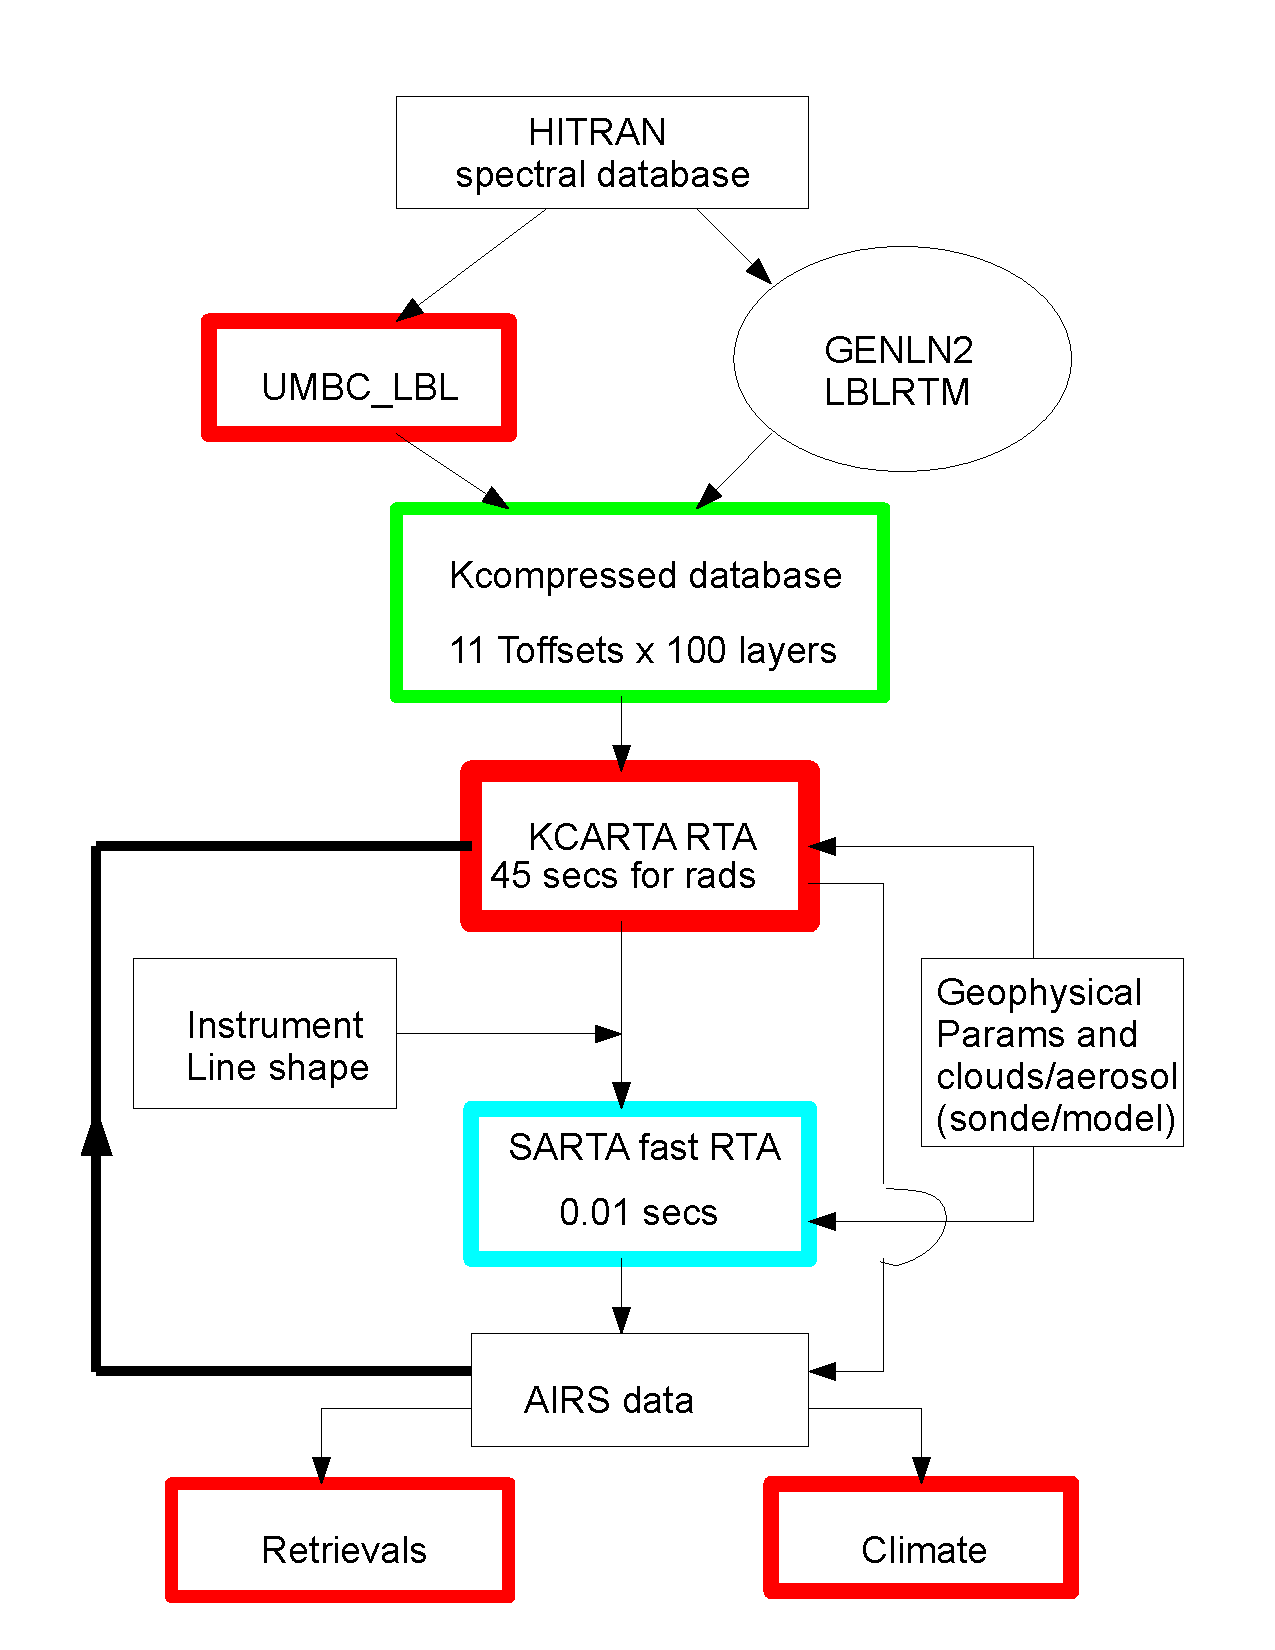
\includegraphics[width=0.5\textwidth]{kcarta_sarta.pdf}
%   \end{center}
% \end{frame}

%%%%%%%%%%%%%%%%%%%%%%%%%%%%%%%%%%%%%%%%%%%%%%%%%%%%%%%%%%%%%%%%%%%%%%%%
\section{kCARTA}
\begin{frame}
  \frametitle{KCARTA Details}
  \begin{itemize}
  \item Uses various HITRAN databases and water continuum models
  \item In addition to IR Sounder Spectral region we have 15-605 \wn, 2830-44000 \wn capability
  \item Clear/cloudy sky calculation includes fast analytic jacobians
  \item Background thermal done at each layer/wavenumber point with
    variable diffusivity angle
  \item Fluxes/heating rates can be computed
  \end{itemize}
\end{frame}
% -------------------------------------------------------------------------------------
\begin{frame}
  \frametitle{kCARTA Development: Continual!}
  \vspace{-0.15in} \small\textcolor{blue}{(blue = under development)}

  {\bf \textcolor{maroon}{Have continually updated kCARTA with each HITRAN
      release} } \vspace{-0.1in}

  \begin{small}
    \begin{itemize} \itemsep0.25pt
    \item Past: 1996,2000,2004,2008,2012 .. \textcolor{maroon}{now have
        2016}
    \item Recent addition: GEISA 2015 (European ``HITRAN'')

    \end{itemize}
  \end{small}

  \textcolor{maroon}{\water : }"without basement" plus continuum (MT-CKD
  2.5, 3.2) \vspace{-0.1in}
  \begin{small}
    \begin{itemize} \itemsep0.25pt
    \item \textcolor{blue}{kCARTA has HDO; will break out HDO scaling for
        future SARTAs}
    \end{itemize}
  \end{small}

  \textcolor{maroon}{\cd :} UMBC line mixing based on 1998 data/HITRAN
  \vspace{-0.1in}
  \begin{small}
    \begin{itemize} \itemsep0.25pt
    \item Can use LBLRTM \cd line mixing, v12.4, 12.8, (from Hartmann)
    \item \textcolor{blue}{HITRAN now provides line mixing package from
        Hartmann, we found problems that HITRAN is fixing.}  Hopefully
      soon!
    \item \textcolor{blue}{non-LTE fitting} : Updated for HITRAN 2016
    \item \textcolor{blue}{4.3 $\mu$m collision induced absorption:
        \cd:\nitrogen, and now \cd:\water Hartmann}
    \end{itemize}
  \end{small}

  \textcolor{maroon}{\methane : } Our LBL code defaults to Voigt lineshape
  \vspace{-0.1in}
  \begin{small}
    \begin{itemize} \itemsep0.25pt
    \item LBLRTM has \methane line mixing, now used in SARTA
    \end{itemize}
  \end{small}

\end{frame}
% -------------------------------------------------------------------------------------
\subsection{Uncertainities}
\begin{frame}
  \frametitle{Comparing \cd line mixing, \water databases}

  % \hspace{0.5in} \emph{\cd 15$\mu$m} \hspace{1.5in} \emph{\water
  % 6.7$\mu$m}\\
  % \begin{center}
  %   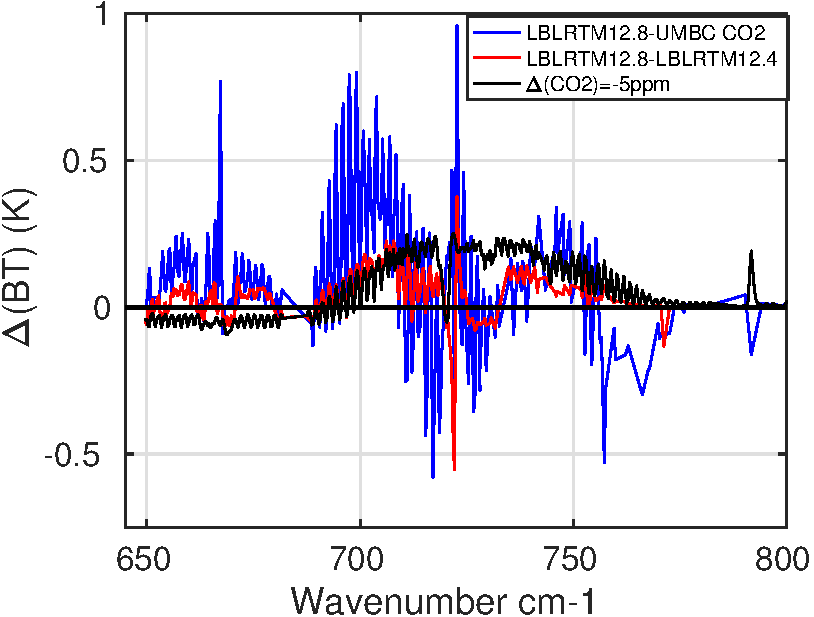
\includegraphics[width=0.48\linewidth]{Figs/FigsHITRAN/co2_intercompare_different_models2.pdf}
  %   \hfill
  %   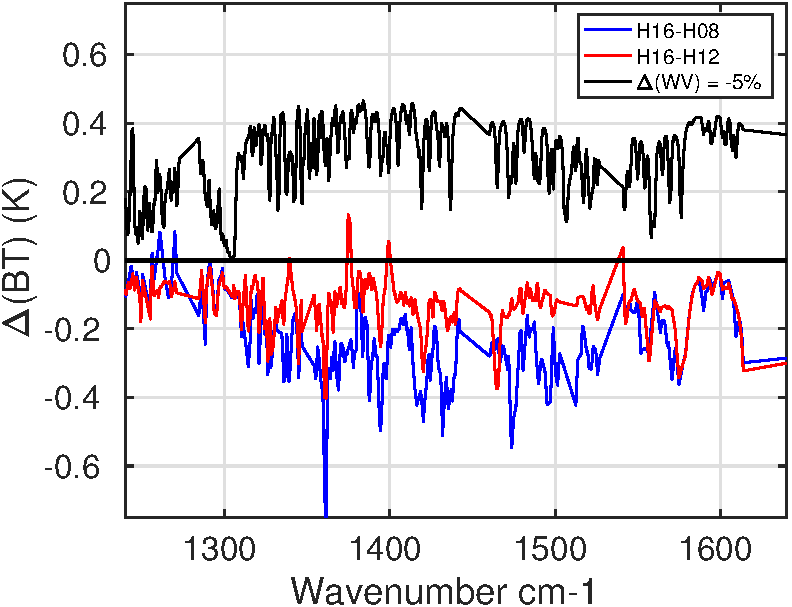
\includegraphics[width=0.48\linewidth]{Figs/FigsHITRAN/wv_intercompare_different_models2.pdf}
  % \end{center}



  \begin{columns}

    \begin{column}{0.55\columnwidth}
      \begin{block}{\hspace{0.2in}\cd 15$\mu$m}
        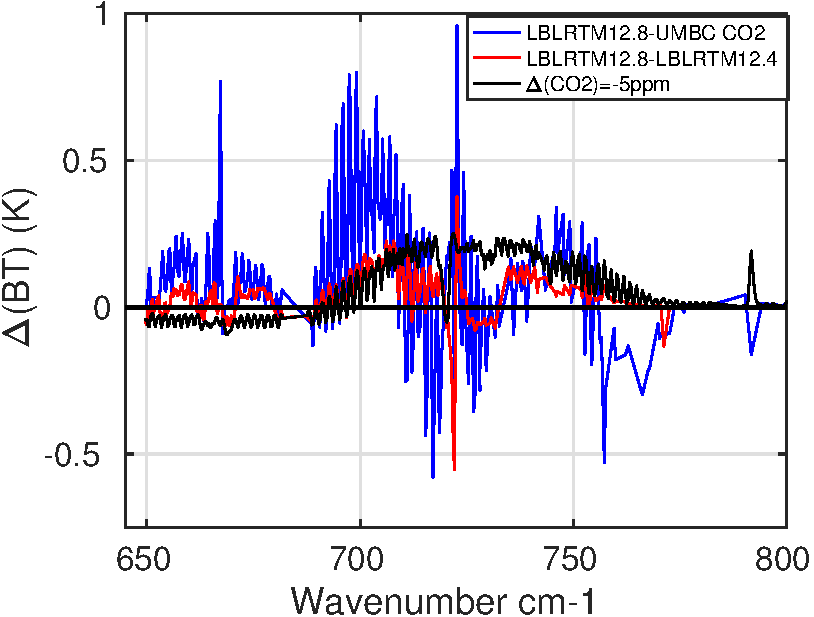
\includegraphics[width=\linewidth]{Figs/FigsHITRAN/co2_intercompare_different_models2.pdf}
      \end{block}
    \end{column}

    \begin{column}{0.55\columnwidth}
      \begin{block}{\hspace{0.2in}\water 6.7$\mu$m}
        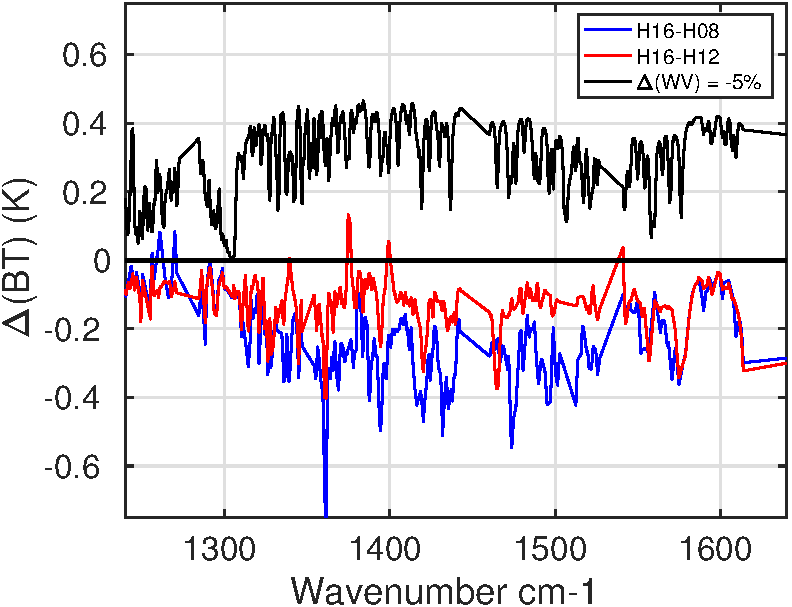
\includegraphics[width=\linewidth]{Figs/FigsHITRAN/wv_intercompare_different_models2.pdf}
      \end{block}
    \end{column}

  \end{columns}

\end{frame}

\begin{frame}
  \frametitle{Assessing \methane line mixing, HITRAN 2016 vs GEISA 2015}

  % \begin{columns}[T] % align columns
  %   \begin{column}{.48\textwidth}
  %     \centering
  %     \textbf{\methane line mixing} \\
  %     LBLRTM has \methane line mixing (H2012), we do not (H2016)
  %   \end{column}
  %   \hfill
  %   \begin{column}{.48\textwidth}
  %     \textbf{HITRAN-16 vs GEISA-15}\\
  %     Not all xsec gases that I use are in GEISA (will soon be fixed)
  %   \end{column}
  % \end{columns}

  % \vspace{0.25in}
  % 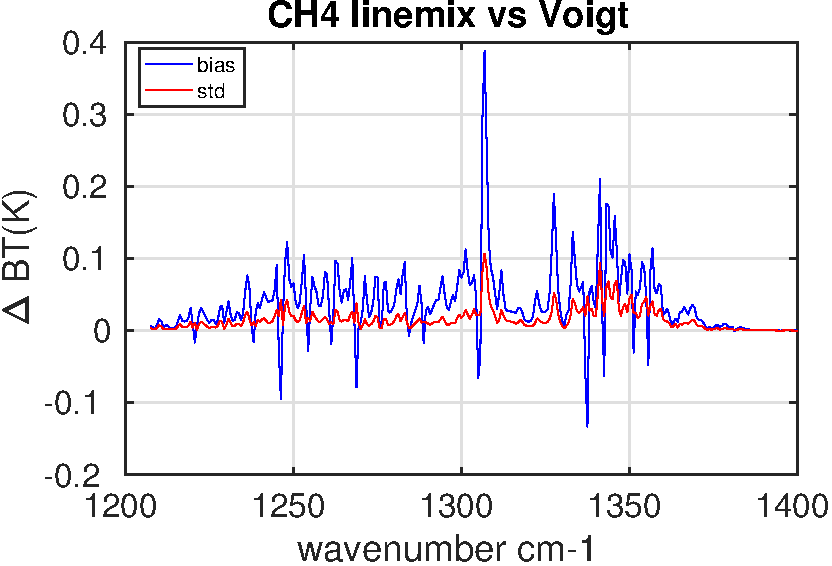
\includegraphics[width=0.48\textwidth]{Figs/FigsH16_G15/ch4linemix2.pdf}
  % 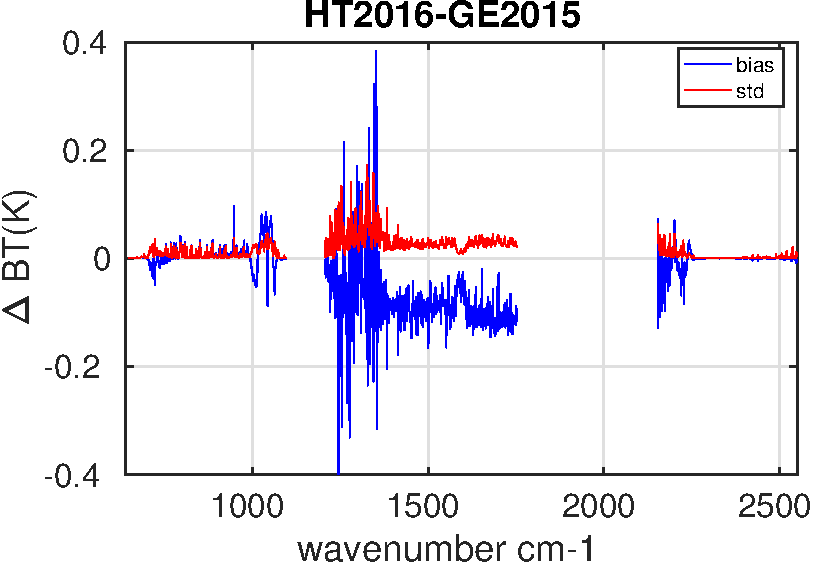
\includegraphics[width=0.48\textwidth]{Figs/FigsH16_G15/h16_g15_v2.pdf}

  \begin{columns}

    \begin{column}{0.55\columnwidth}
      \begin{block}{\methane line mixing}
        \small  LBLRTM has \methane line mixing (H2012), we do not (H2016)\\
        \vspace{0.2in}
        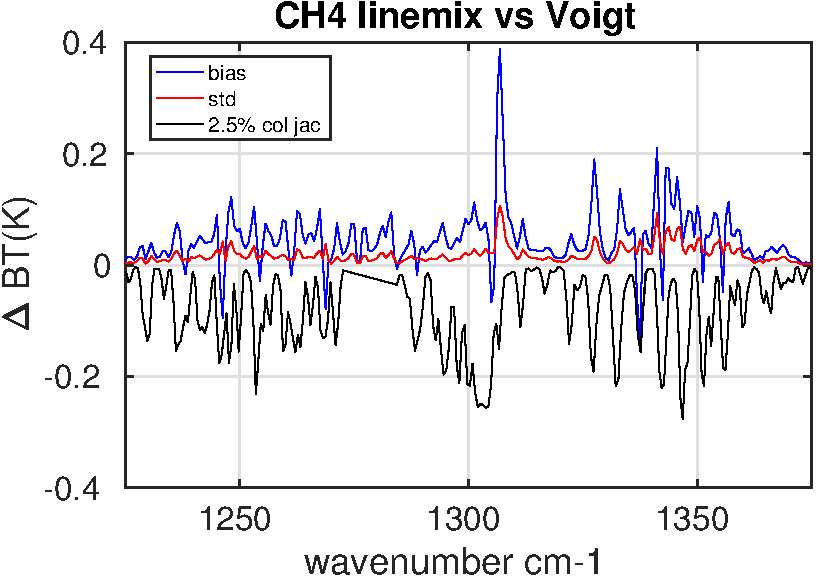
\includegraphics[width=\linewidth]{Figs/FigsH16_G15/ch4linemix3.pdf}
      \end{block}
    \end{column}

    \begin{column}{0.55\columnwidth}
      \begin{block}{HITRAN-16 vs GEISA-15}
        \small   Not all xsec gases that I use are in GEISA (will soon be fixed)\\
        \vspace{0.2in}
        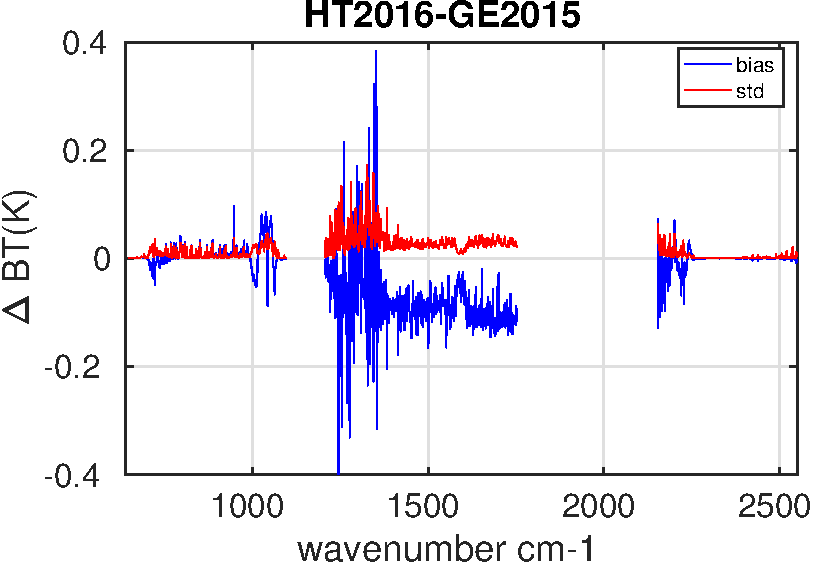
\includegraphics[width=\linewidth]{Figs/FigsH16_G15/h16_g15_v2.pdf}
      \end{block}
    \end{column}

  \end{columns}


      
\end{frame}

%%%%%%%%%%%%%%%%%%%%%%%%%%%%%%%%%%%%%%%%%%%%%%%%%%%%%%%%%%%%%%%%%%%%%%%%
\section{SARTA}
% --------------------------------------------------------------------
\begin{frame}\frametitle{Fast Radiative Transfer (SARTA)}
  \begin{itemize}
  \item Validated against kCARTA LBL and statistical analysis of large test
    data sets.
  \item Allows computation of SARTA error covariance matrix (for
    parmeterization errors)
  \item Clear/cloudy RT calcs using eg sonde (clear) or NWP model fields
    (cloudy)
  \item Many minor gases included
  \item Emissivity and reflectance
    \begin{itemize}
    \item Ocean emissivity by Masuda (wind speed dependance)
    \item Land emiss by U. Wisc or NASA Langley
    \item \textcolor{blue}{Daytime over ocean bi-directional reflectance
        (Nalli et. al.)}
    \end{itemize}
  \end{itemize}
\end{frame}
% --------------------------------------------------------------------
\begin{frame}
  \frametitle{Latest CrIS FSR SARTA}
  Already delivered
  
  \begin{itemize}
  \item HITRAN 2012 (molecular and xsec gases)
  \item MT-CKD 2.5
  \item LBLRTM v12.4 : \cd and \methane line mixing
  \end{itemize}

  Future plans (roughly ordered by increasing complexity)
  \begin{itemize}
  \item \amm + MT-CKD3.2 + HITRAN2016
  \item HDO (column mult wrt \water is easy; 100 layer more involved)
  \item Updated \cd line mixing (depends on kCARTA tests)
  \item 4.3 um bandhead \cd/\water and \cd/\nitrogen CIA (depends on kCARTA
    tests)
  \item Move from linear regression to Gaussian Kernel Regression?
    \begin{itemize}
    \item LLS is straighforward but can be inaccurate ``outside training''
    \item GKR is more accurate esp ``outside training'' regime; very
      promising but much more complex
    \end{itemize}
  \item \textcolor{blue}{New parameterization with simplified algorithm
      (longer term)}
  \end{itemize}
  
\end{frame}

\begin{frame}
  \frametitle{New Spectroscopy For LBL (J.M. Hartmann/H. Tran)}
  \vspace{-0.1in} Recent work by J.M. Hartmann/H. Tran and others (HITRAN
  2018 Conference) indicate that N$_2$-\water and \cd-\water collisions are
  important for the 4.3 $\mu$m band head!  Significant effort to
  incorporate into LBL and separate from existing \water continuum.

  \vspace{-0.1in}
  \begin{columns}

    \begin{column}{0.55\columnwidth}
      \begin{block}{Lab Spectra}
        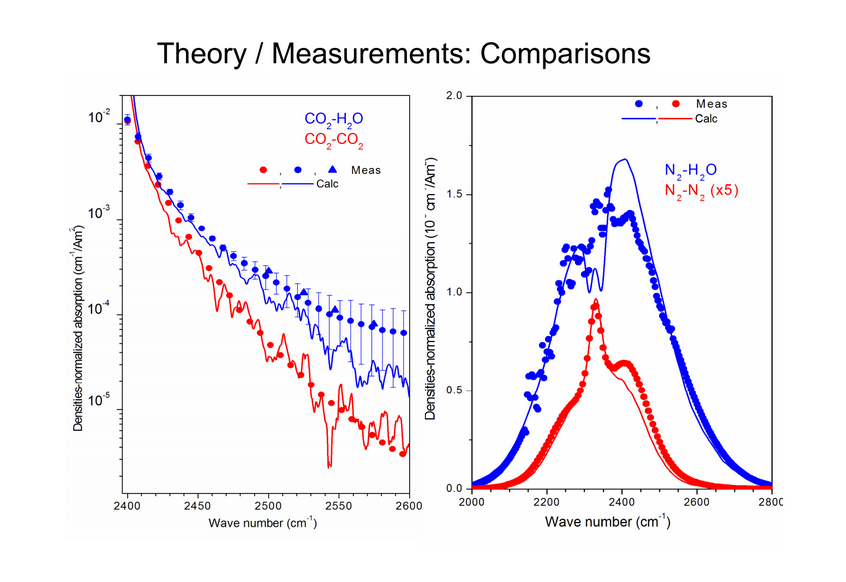
\includegraphics[width=\linewidth]{HartmannSlide1.png}
      \end{block}
    \end{column}

    \begin{column}{0.55\columnwidth}
      \begin{block}{IASI Biases}
        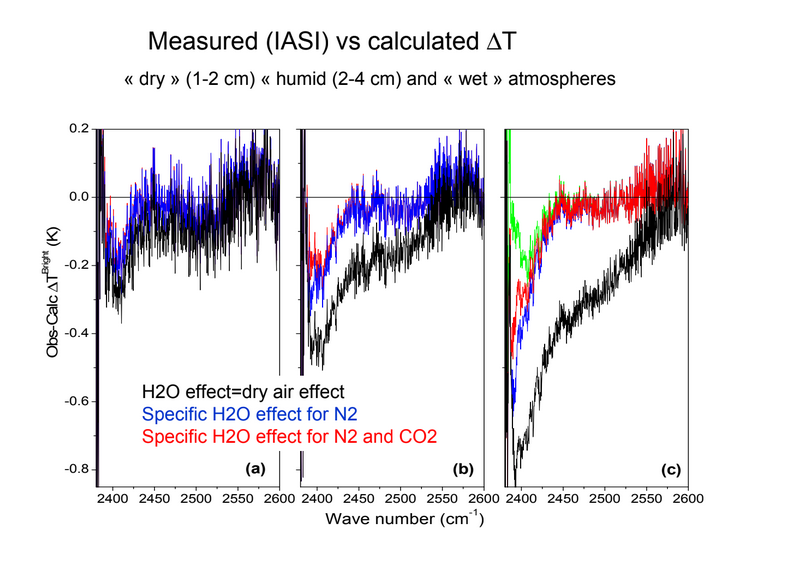
\includegraphics[width=\linewidth]{HartmannSlide2.png}
      \end{block}
    \end{column}

  \end{columns}

\end{frame}

% --------------------------------------------------------------------
\begin{frame}\frametitle{SARTA vs kCARTA comparison (49 regr profiles)}
  \centering
  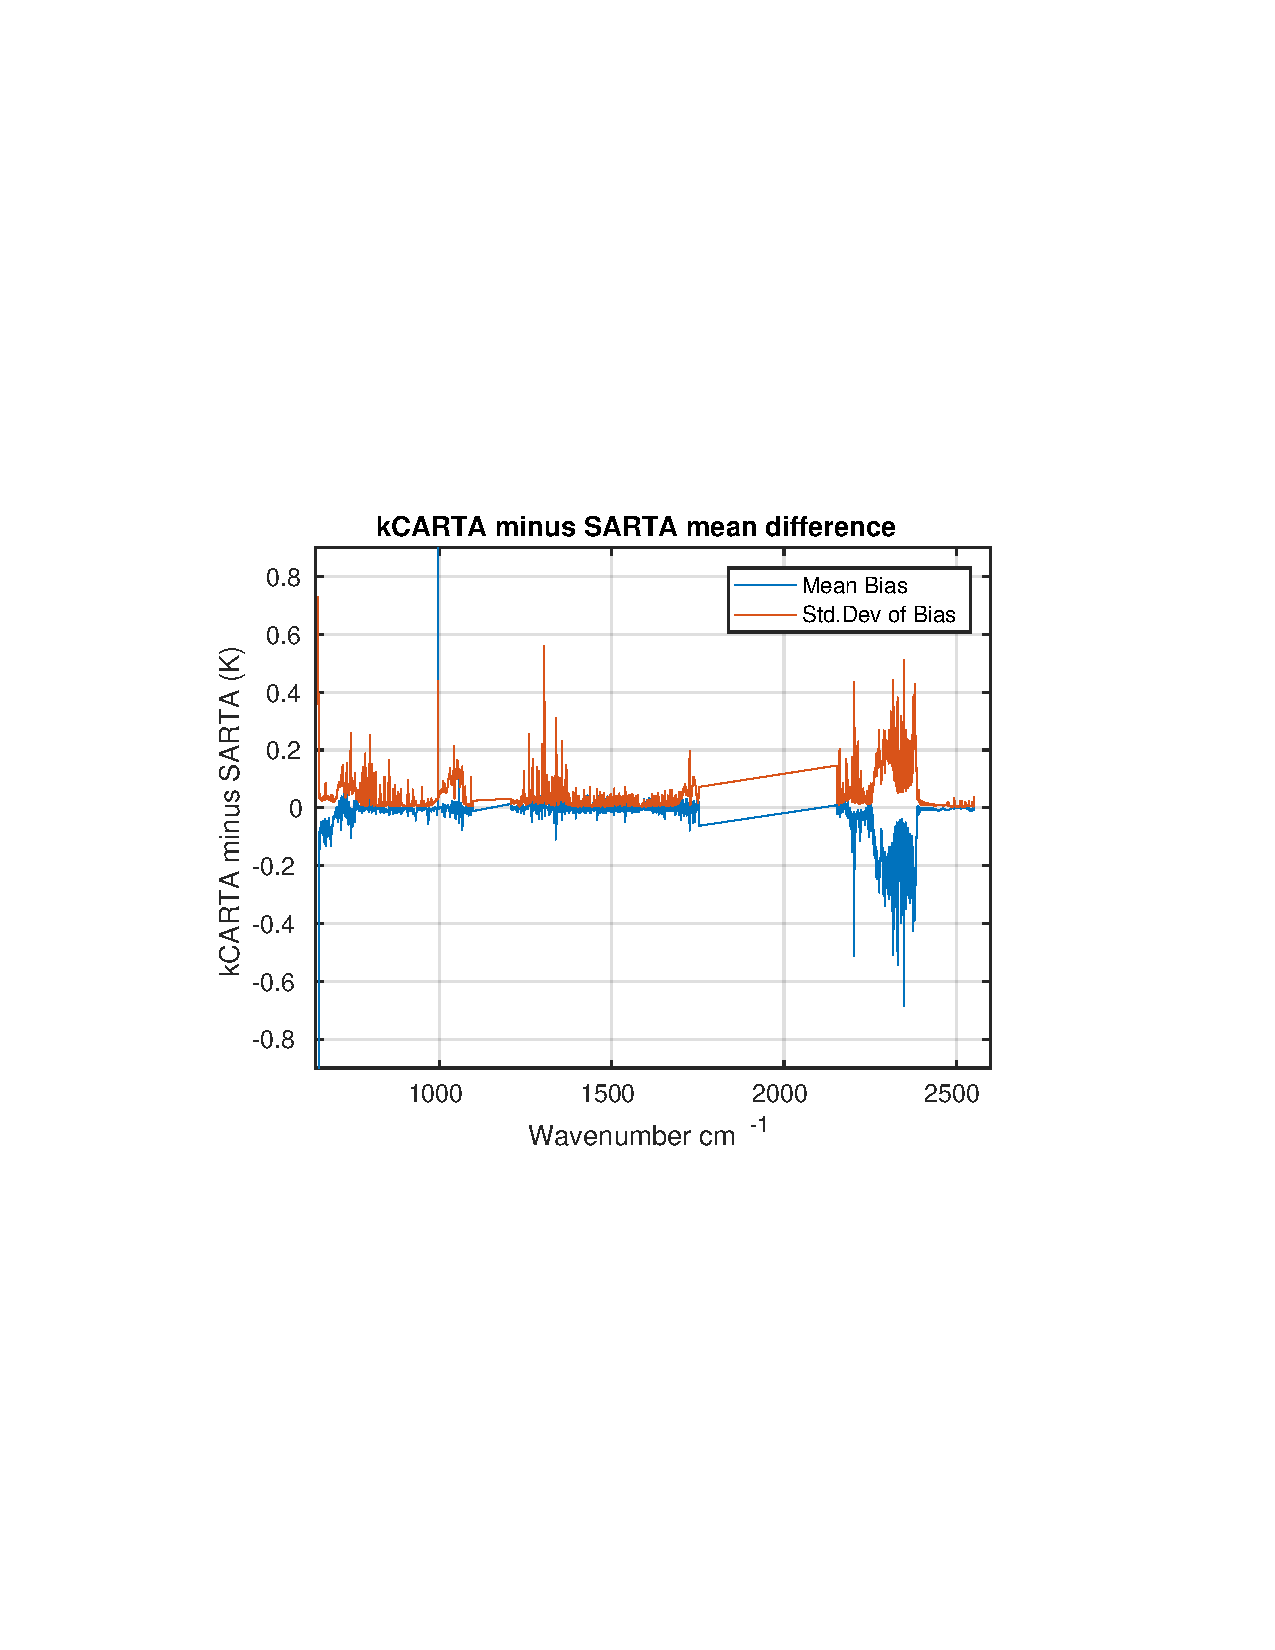
\includegraphics[width=0.95\linewidth]{./r49_kcarta_sarta_bias_std_spectrum.pdf}
\end{frame}
% --------------------------------------------------------------------
\begin{frame}\frametitle{\amm : SARTA vs KCARTA}
  \centering
  % 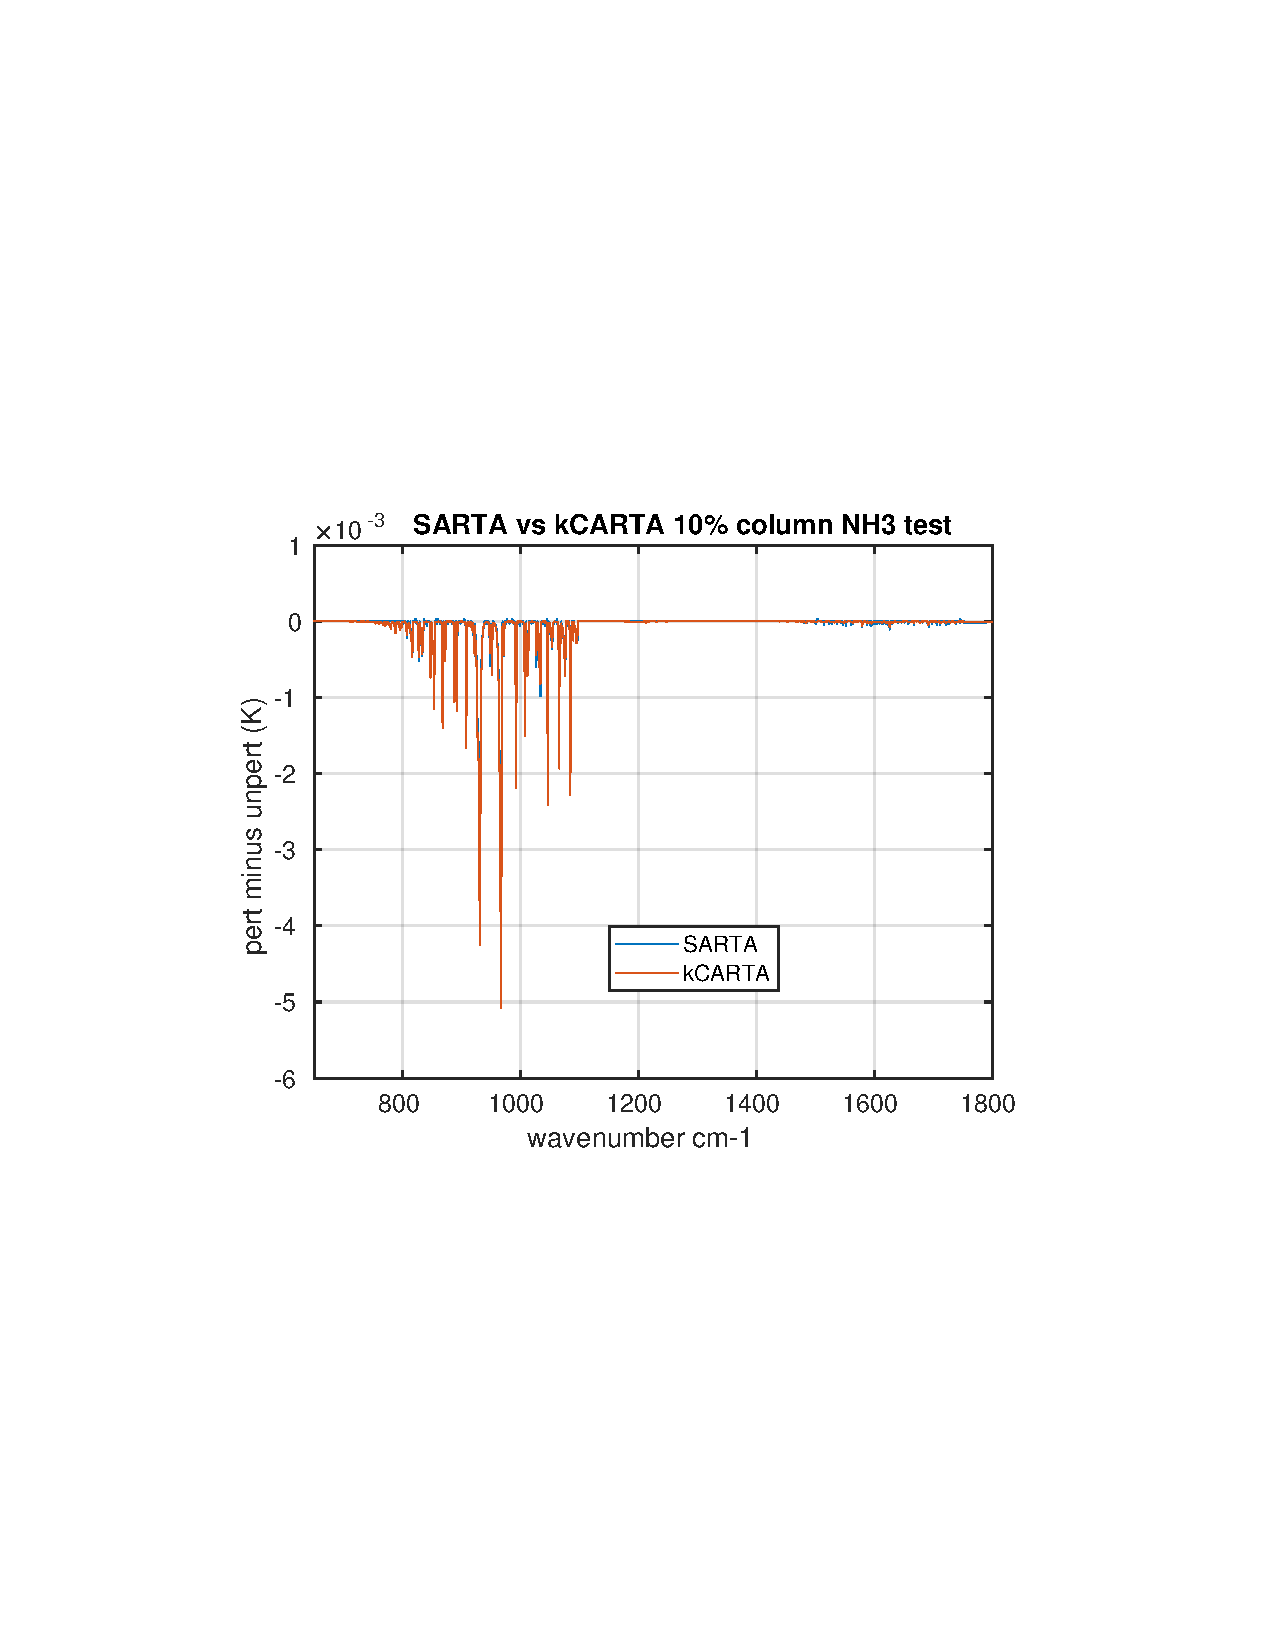
\includegraphics[width=0.9\linewidth]{./sarta_kcarta_nh3_perturb_unitemis.pdf}
  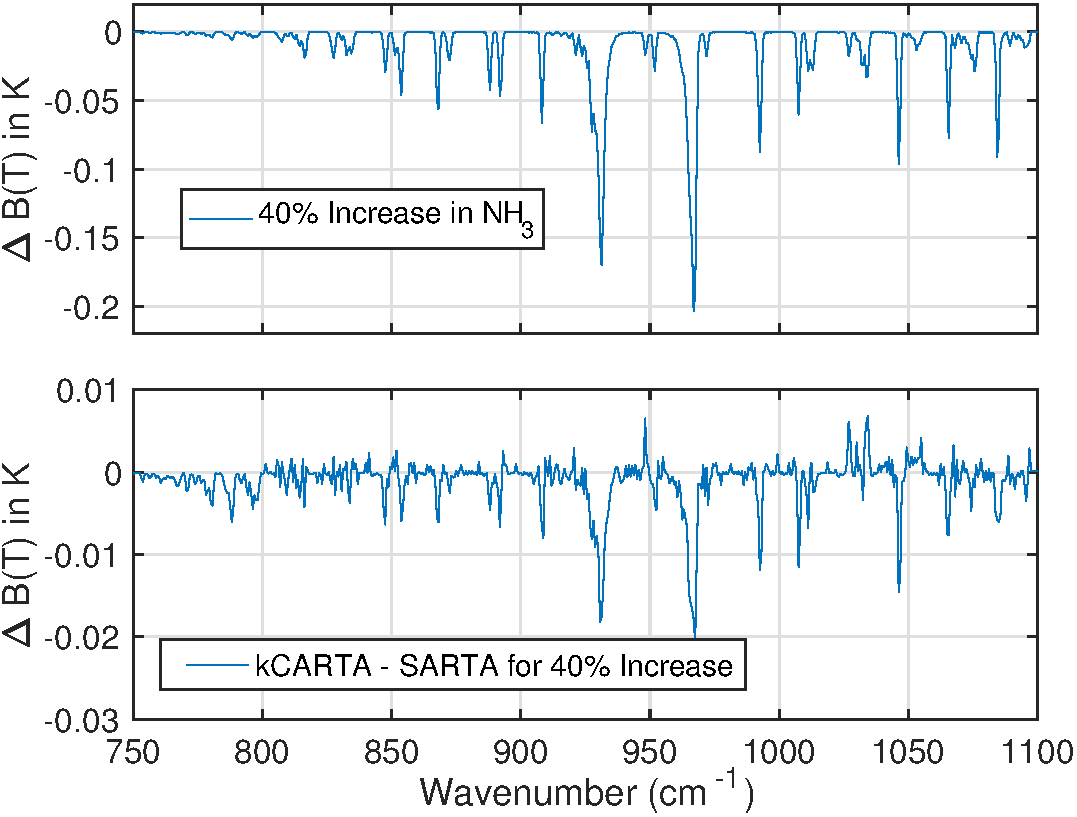
\includegraphics[width=0.9\linewidth]{lls_nh3.pdf} \newline Small, mostly
  systematic errors (4\% error for 40\% variation in \amm).
\end{frame}
% --------------------------------------------------------------------

%%%%%%%%%%%%%%%%%%%%%%%%%%%%%%%%%%%%%%%%%%%%%%%%%%%%%%%%%%%%%%%%%%%%%%%%
\section{Retrievals}

\begin{frame}
  \frametitle{Single Footprint Retrievals}
  \begin{itemize}
  \item Cloud Representation : NWP multilayer cloud converted to Two Slab
    Clouds (ice/water)
    \begin{itemize}
    \item OEM methodology, so DOF is a natural diagnostic
    \item smoothing by combination of Tikonov matrices,
      $\sigma(i)^2 e^{-((i-j)/h)^2}$, climatology
    \item State vector : Surf temp, \textcolor{red}{100 layer}
      T(z),\water(z),O3(z),\textcolor{red}{ice and water clouds}
    \item \textcolor{red}{100 layer retrieval takes $\le$ 2 seconds per
        single FOV}
    \end{itemize}
  \end{itemize}

  \begin{columns}[T] % align columns
    \begin{column}{.38\textwidth}

\small

      Single Footprint Retrievals, DeSouza-Machado {\em et. al., Atmos. Meas. Tech.}, 2018 \newline
      %https://doi.org/10.5194/amt-11-529-2018

      Evaluation of Radiative Transfer Models with Clouds, Aumann {\em et. al., J. Geophys. Res},2018
      %\newline 10.1029/2017JD028063

\end{column}%
\hfill%
\begin{column}{.58\textwidth}

  \centering
  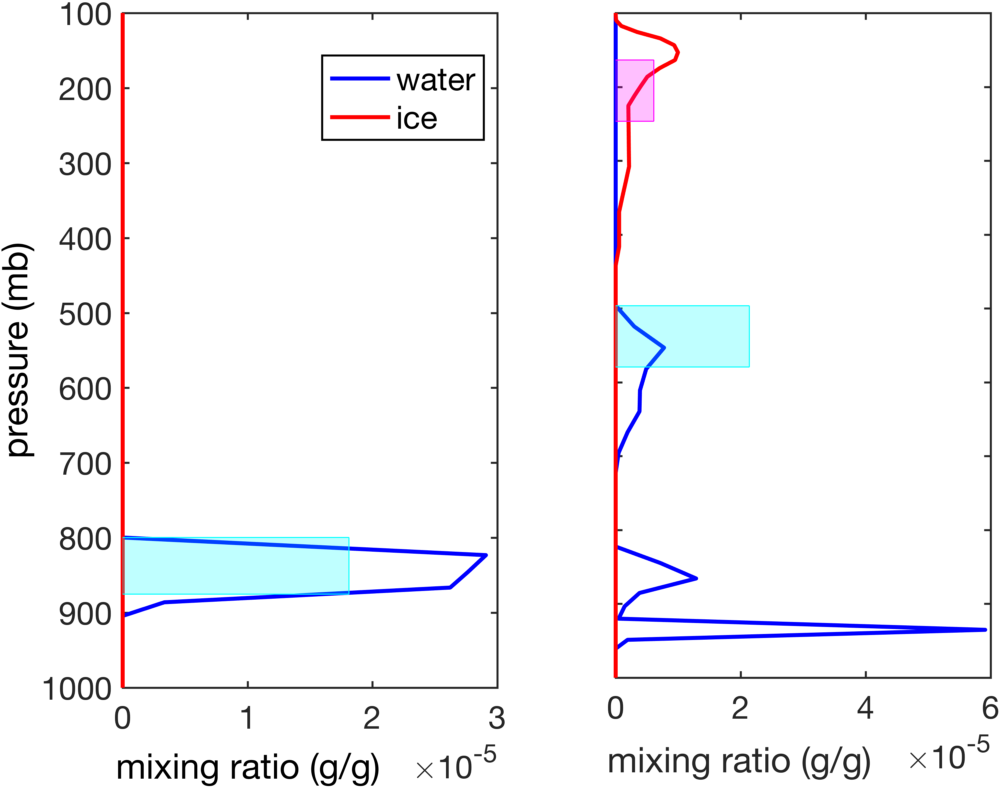
\includegraphics[width=0.75\linewidth]{Figs/FigsRetr/clouds_profileG040_271_321_lls.png}
\end{column}%
\end{columns}

\end{frame}

\begin{frame}
  \frametitle{Ice Cloud ODs 2011/03/11 day}

  \hspace{0.50in} AIRS L2 \hspace{1.75in} UMBC \\
  \begin{center}
    \dlandgraph{0.48}{Figs/FigsRetr/JPL_Feb2018_CompareMagicSonde/kahn_iceOD_day_2011_03_11_log.pdf}{Figs/FigsRetr/JPL_Feb2018_CompareMagicSonde/umbc_iceOD_day_2011_03_11_log.pdf}
  \end{center}

  Have looked at cldforcing, and the differences in cloud OD (UMBC vs L2)
  are typically in regions of "low" forcing, need to investigate further

\end{frame}

\begin{frame}
  \frametitle{Water Cloud ODs 2011/03/11 day}
  % \emph{note the colorbar for MODIS L3 spans a wider range}\\
  (different sensor/wavelengths used in retrieval, so expect different
  magnitude ODs ... but patterns are similar)

  \hspace{0.50in} MODIS L3 \hspace{1.75in} UMBC \\
  \begin{center}
    \dlandgraph{0.48}{Figs/FigsRetr/JPL_Feb2018_CompareMagicSonde/modisL3_waterOD_day_2011_03_11_log.pdf}{Figs/FigsRetr/JPL_Feb2018_CompareMagicSonde/umbc_waterOD_day_2011_03_11_log.pdf}
  \end{center}
\end{frame}

\begin{frame}
  \frametitle{2011/03/11 g039 : DCC over TWP}

  \noindent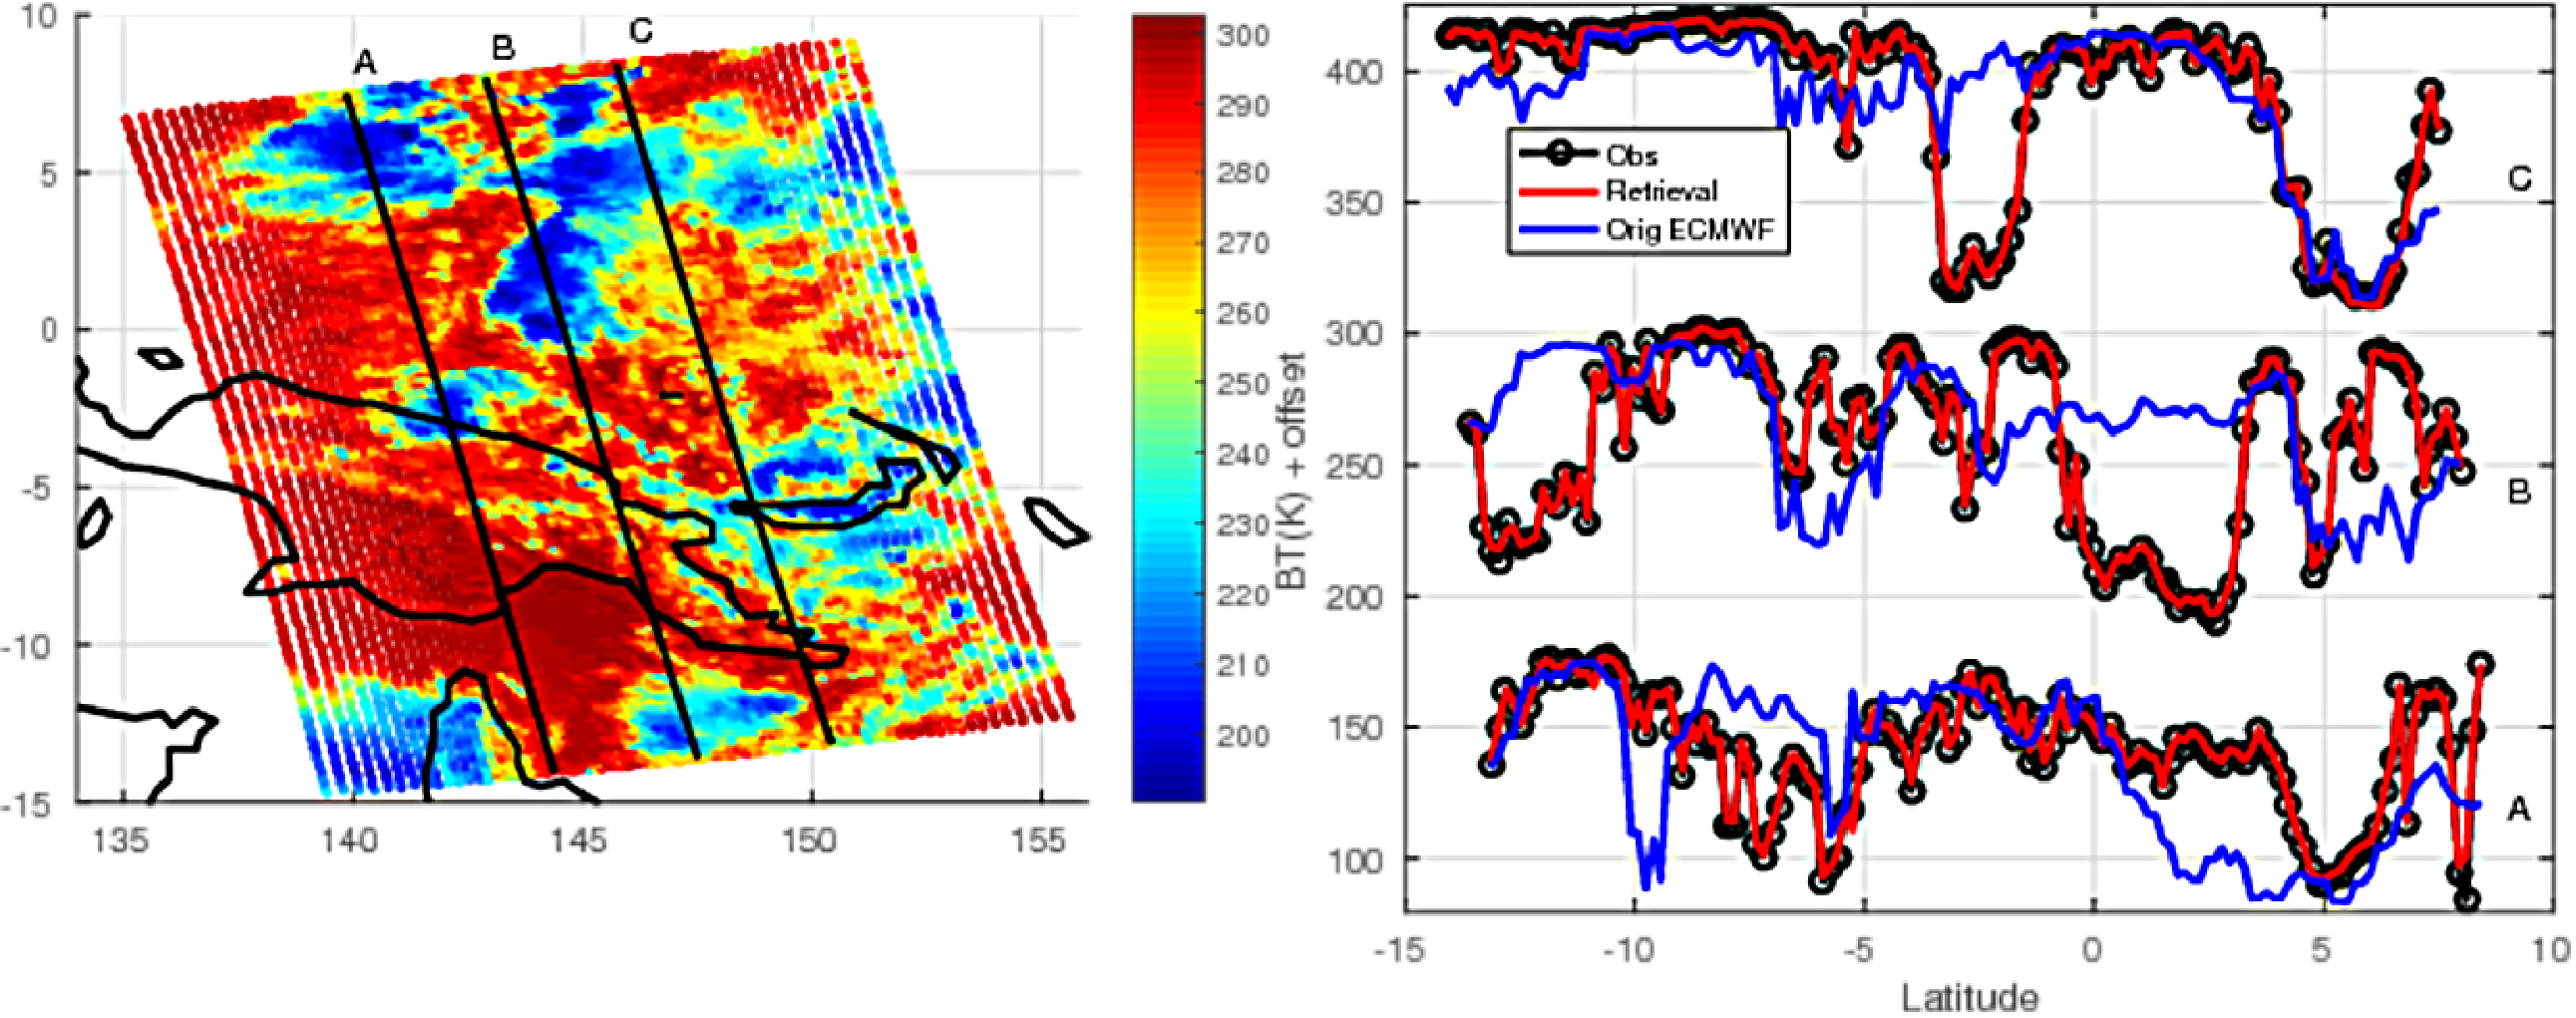
\includegraphics[width=\textwidth]{Figs/FigsRetr/AIRS_STM_Apr17/gran039_2011_03_11_bt1231_scatter_obs_3lines.pdf}

  BT 1231 \wn observations and calculations, in Kelvin.\newline

  \vspace{-0.2in} Left panel : AIRS observations for Granule 039 on March
  11, 2011. The lines are at three different AIRS scan angles. \newline

  \vspace{-0.2in} Right panel : BT1231 Observations (black) compared to
  calculations using the original ECMWF model fields (blue) and with the
  mitigated/retrieved cloud fields (red).
	 
\end{frame}

%%%%%%%%%%%%%%%%%%%%%%%%%

\begin{frame}
  \frametitle{Ice CldTop Heights}

  \hspace{0.25in} ECMWF \hspace{1.00in} UMBC retr \hspace{1.0in} MODIS L2  \\
  \begin{center}
    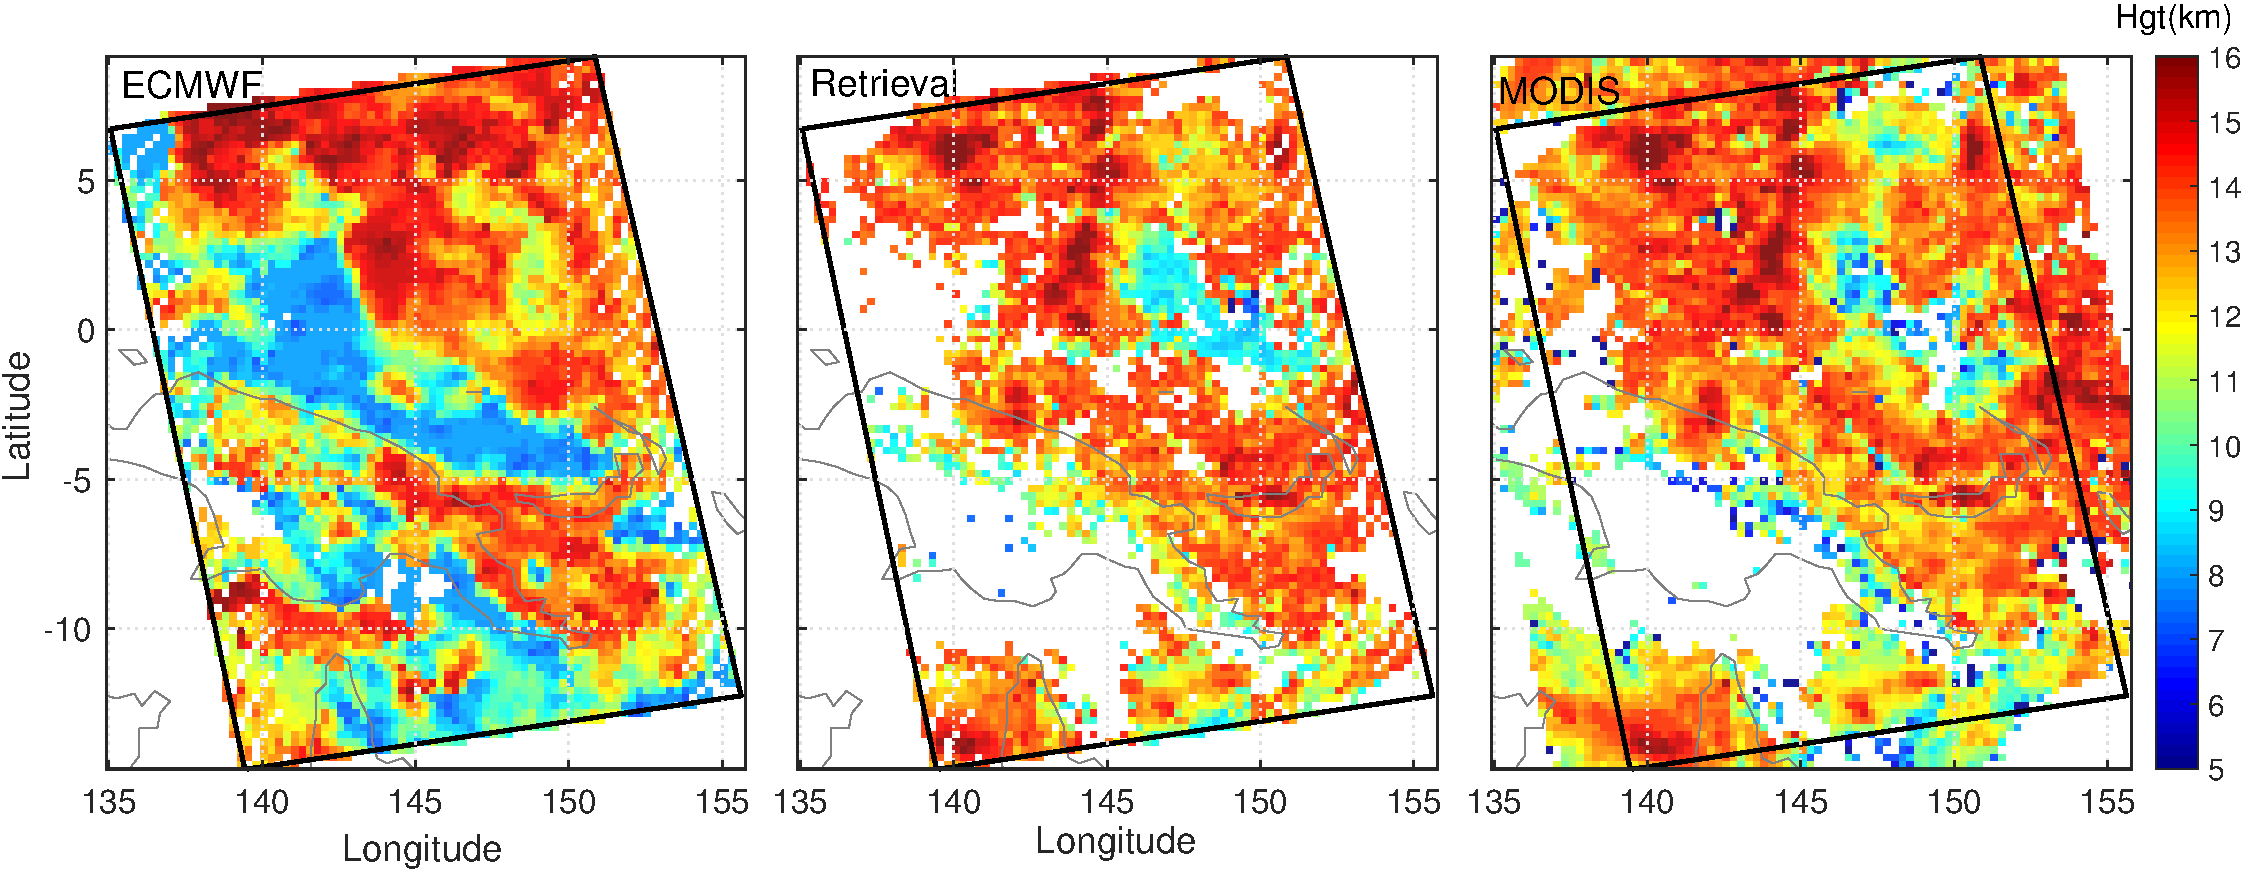
\includegraphics[width=0.95\linewidth]{Figs/FigsRetr/cldheight_v2.pdf}
  \end{center}

  Ice clouds with OD $\le$ 0.5 have been removed from plots \\
  Note similarity to BT1231 obs (high clouds = cold obs)
  
\end{frame}


\begin{frame}
  \frametitle{DOFS and ice OD comparisons}

  \hspace{0.50in} DOFS \hspace{1.75in} Ice OD  \\
  \begin{center}
    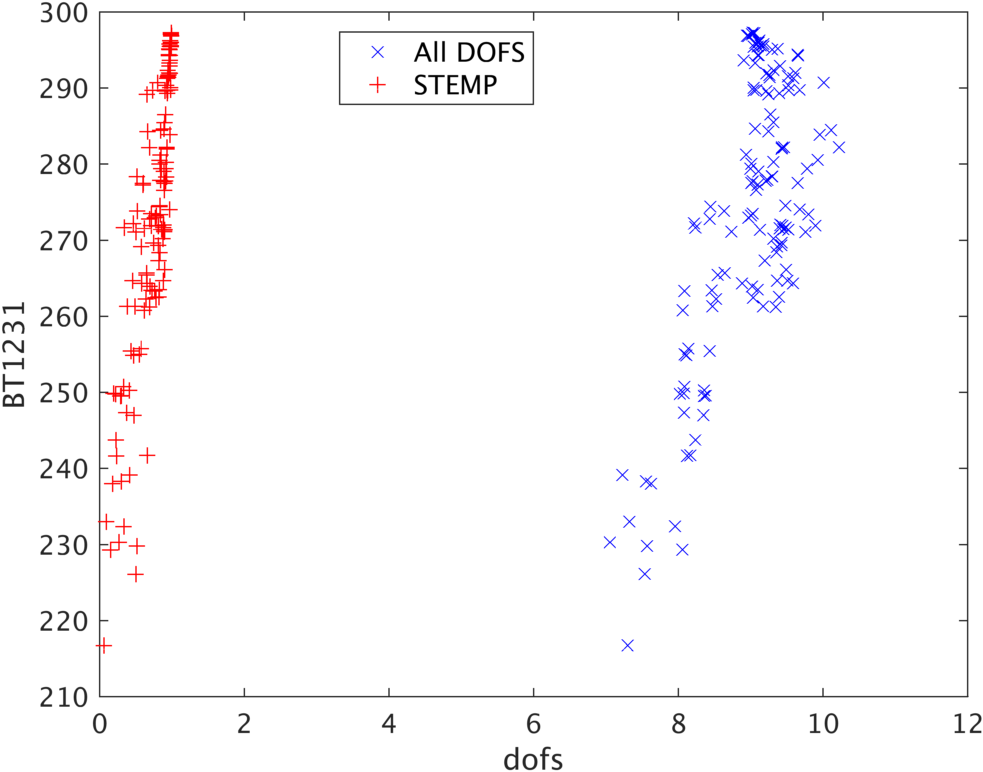
\includegraphics[width=0.45\linewidth]{Figs/FigsRetr/AIRS_STM_Apr17/dofs_all_stemp_2011_03_11.png}
    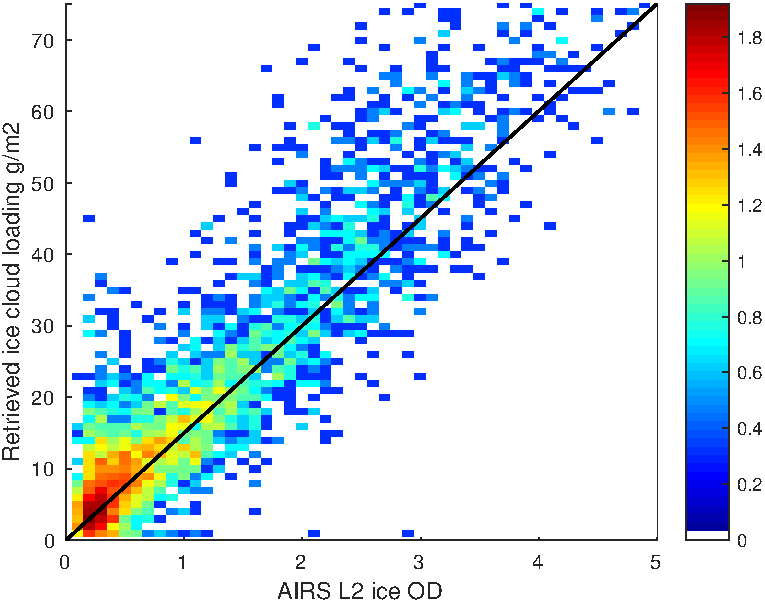
\includegraphics[width=0.45\linewidth]{Figs/FigsRetr/AIRS_STM_Apr17/cloud1_OD_G039_new_may23_2016.pdf}
  \end{center}

  DOF scale with obs BT 1231 : \textcolor{red}{Red crosses for stemp
    (between 0 and 1)}, \textcolor{blue}{blue crosses : all DOF (between 6
    and 14)}

  Ice OD : UMBC cloud loading vs AIRS L2 : colorbar is log10(number of
  points)

\end{frame}

%%%%%%%%%%%%%%%%%%%%%%%%%
\begin{frame}
  \frametitle{Lindenberg, Germany GRUAN sondes \newline 52.21N, 14.12 E, 98
    m asl}

  \begin{itemize}
  \item 3200 sonde launches over a few years, ($\sim$ 220 each month)
  \item Select AIRS ovepasses within $\pm$ 1 hour and 100 km of sonde
    launch, gives 80-100 "nearest" AIRS obs per sonde
  \item Match AIRS observations to ERA thermodynamic/cloud profiles (252455
    "nearest" AIRS obs)
  \item Compare retrievals to sonde, sonde*AK and ERA
  \item Look at results as function of DOF
  \end{itemize}

  \vspace{0.125in} Wide variety of atmospheric conditions
  \begin{itemize}
  \item Surf temp varies from from 275 K (winter) to 295 K (summer); col
    water from 8 to 26 mm
  \item Clouds varied from none to DCC : Mean cloud forcing each month
    (Surftemp-BT1231 obs) = 15 K
  \end{itemize}
\end{frame}

\begin{frame}
  \frametitle{Sonde-UMBC Retrieval}
  Divide the retrievals in quantiles of DOF, look at 4 quantile ranges\\

  \begin{small}
    \begin{table}[h]
      \begin{center}
        \begin{tabular}{lcccc}
          \hline
          Cloud     & Quantile & DOF range & CldEffect(K) &  Number \\
          condition & range    &           & (rough)      & AIRS obs \\
          \hline
          Very Thick cloud & 0.0-0.1 & 0.00-3.12 & > 50  & 2769 \\
          Thick cloud      & 0.1-0.5 & 3.12-4.29 & 20-50 & 43699 \\
          Medium Cloud     & 0.5-0.9 & 4.29-6.84 & 2-20  & 84579 \\
          Thin/no cloud    & 0.9-1.0 & 6.38-8.65 & < 2 & 24742 \\
          \hline
        \end{tabular}
      \end{center}
    \end{table}
  \end{small}

  \begin{center}
    \noindent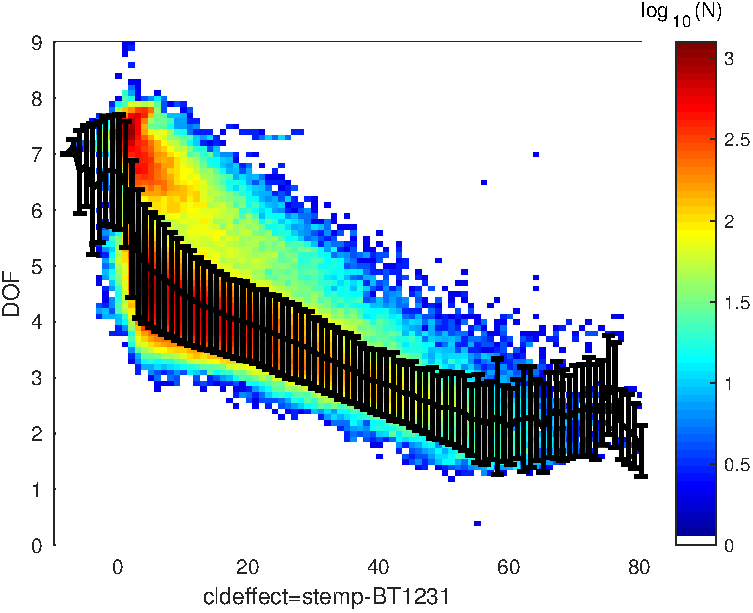
\includegraphics[width=0.45\textwidth]{Figs/FigsRetr/AIRS_STM_Apr18/dofs_vs_cldeffect_iSondeList_5_iStemp_ColWV_4_xvers_5_iSubset_1_dofALL.pdf}
  \end{center}
\end{frame}
% 0-0.1 (thick cloud), 0.1-0.5 (medium/thick clouds) 0.5-0.9 (thin cloud) 0.9-1.0 (almost clear)\\
% 0-3.12 (2769), 3.12-4.29 (43699),4.29-6.84(84579),6.38-8.65(24742)

\begin{frame}
  \frametitle{Sonde-UMBC Retrieval}
  Divide the retrievals in quantiles of DOF, look at 4 quantile ranges\\
  \textcolor{red}{As expected biggest problems when clouds are thickest
    (low DOF)}; otherwise <sonde-retrieval> is typically within 1 K, 20\%
  RH

  \vspace{0.1in}
  T(z)  \hspace{3.0in} RH(z) \\
  \begin{center}
    \dlandgraph{0.48}{Figs/FigsRetr/AIRS_STM_Apr18/deltaTz_iSondeList_5_iStemp_ColWV_4_xvers_5_iSubset_1_dofALL.pdf}{Figs/FigsRetr/AIRS_STM_Apr18/deltaRHz_iSondeList_5_iStemp_ColWV_4_xvers_5_iSubset_1_dofALL.pdf}
  \end{center}
\end{frame}

%%%%%%%%%%%%%%%%%%%%%%%%%%%%%%%%%%%%%%%%%%%%%%%%%%%%%%%%%%%%%%%%%%%%%%%%
\begin{frame}
  \frametitle{Conclusions}
  \begin{itemize}
  \item We have been concentrating on spectroscopy and line-by-line
    improvements
  \item \cd lineshape changes are particulary important because they are
    \emph{not} static but depend on the \water burden.
  \item We have shown (Lindeberg) that HITRAN 2016 \water is slightly
    better than HITRAN 2012 (not discussed)
  \item Improvement to kCARTA can be migrated to SARTA quickly (with
    current parameterization)
  \item Single Footprint Retrievals are very promising and allow vastly improved validation of SARTA to sondes, reanalysis, etc.  
  \item \textcolor{maroon}{Next delivery : HITRAN16, updated \cd line-mix,
      \amm, HDO}
  \end{itemize}
\end{frame}
\end{document}

%%%%%%%%%%%%%%%%%%%%%%%%%%%%%%%%%%%%%%%%%%%%%%%%%%%%%%%%%%%%%%%%%%%%%%%%
%%%%%%%%%%%%%%%%%%%%%%%%%%%%%%%%%%%%%%%%%%%%%%%%%%%%%%%%%%%%%%%%%%%%%%%%
%%%%%%%%%%%%%%%%%%%%%%%%%%%%%%%%%%%%%%%%%%%%%%%%%%%%%%%%%%%%%%%%%%%%%%%%

%%% Local Variables:
%%% mode: latex
%%% TeX-master: t
%%% End:
